\documentclass[tikz]{standalone}
\usetikzlibrary{fit}
\usetikzlibrary{arrows}

\begin{document}
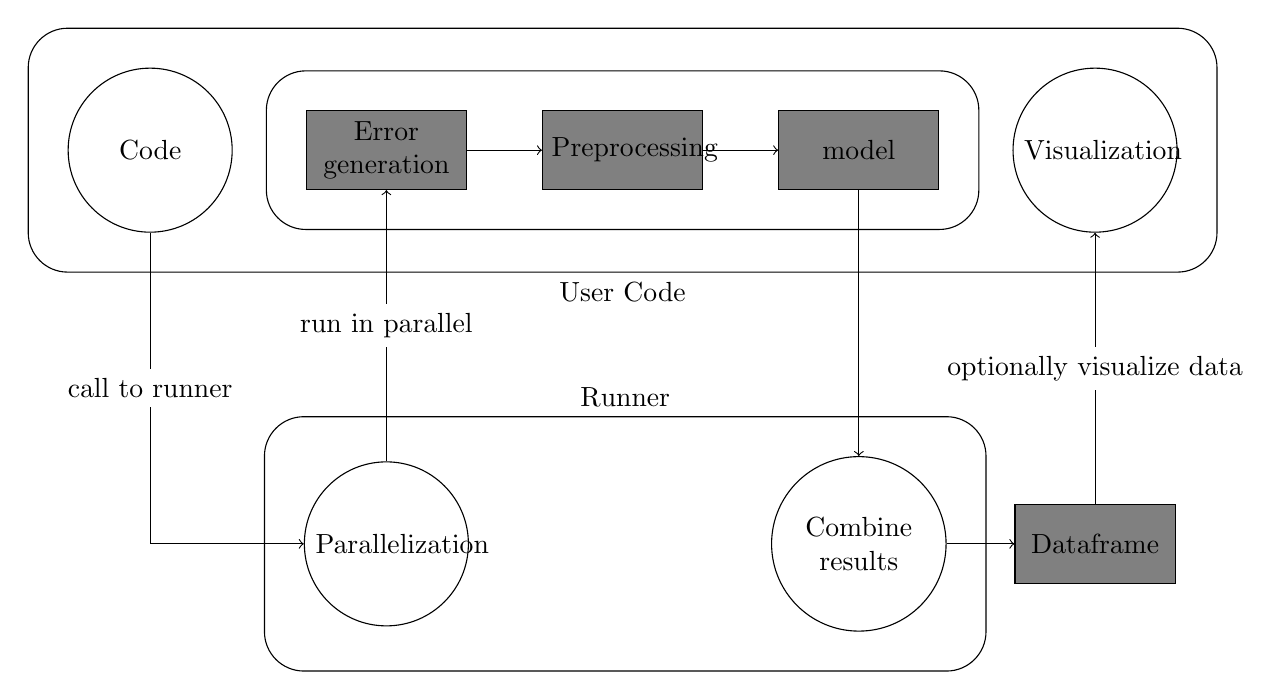
\begin{tikzpicture}[state/.style={circle, draw, align=center, minimum size=1cm, text width=1.8cm},small/.style={circle, draw, align=center, minimum size=1cm, text width=1cm}, file/.style={rectangle, fill=gray, draw, align=center, minimum size=1cm, text width=1.8cm}]
	% nodes
	\node[state] (code) {Code}; %
	\node[file, right of=code, xshift=2cm] (errgen) {Error generation}; %
	\node[state, below of=errgen, yshift=-4cm] (paral) {Parallelization}; %
	\node[file, right of=errgen, xshift=2cm] (preproc) {Preprocessing}; %
	\node[file, right of=preproc, xshift=2cm] (model) {model}; %
	\node[state, below of=model, yshift=-4cm] (combine) {Combine results}; %
	\node[file, right of=combine, xshift=2cm] (data) {Dataframe}; %
	\node[state, right of=model, xshift=2cm] (visual) {Visualization}; %

	% plate
	\node[label=below:User Code, draw, inner sep=.5cm, rounded corners=.5cm, fit=(code)(errgen)(preproc)(model)(visual)] (user) {}; %
	\node[label=above:Runner, draw, inner sep=.5cm, rounded corners=.5cm, fit=(paral)(combine)] (dpemu) {}; %
	\node[draw, inner sep=.5cm, rounded corners=.5cm, fit=(errgen)(preproc)(model)] (runpara) {}; %

	% edges
	\draw [->] (code) |- (paral) node [near start, fill = white] {call to runner};
	\draw [->] (paral) -- (errgen) node [midway, fill = white] {run in parallel};
	\draw [->] (errgen) -- (preproc);
	\draw [->] (preproc) -- (model);
	\draw [->] (model) -- (combine);
	\draw [->] (combine) -- (data);
	\draw [->] (data) -- (visual) node [midway, fill=white] {optionally visualize data};
	% \draw [->] (code) -- +(2cm, 0) |- (preproc) node [near start, fill = white] {$2$};
\end{tikzpicture}
\end{document}
